\documentclass[11pt]{article}
\usepackage[utf8]{inputenc}
\usepackage{caption}
\usepackage{subcaption}


\usepackage{ifpdf}
\ifpdf
\usepackage[pdftex]{graphicx}
\else
\usepackage{graphicx}
\fi

\usepackage[margin=1.25in]{geometry}


\title{6.851 Final Project \\ Tabulation Hashing Performance Benchmark}
\author{Maksim Stephenako \\ Yuzhi Zheng}

\date{May 2012}

\begin{document}


\setlength{\baselineskip}{1.15\baselineskip}

\ifpdf
\DeclareGraphicsExtensions{.pdf, .jpg, .tif}
\else
\DeclareGraphicsExtensions{.eps, .jpg}
\fi

\maketitle

\section{Introduction}
% Yuzhi
Hashing is one of the most basic computer science concept. 
It allows elements to be reliably stored and 
retrieved from a limited number of slots, without dedicated slot of every possible 
variation of the element. While basic, hashing is used everywhere. Hashing is used in 
associative arrays, sometimes also known as dictionaries, in languages like 
PHP, Perl, and Python. Hashing can even be used for database indexing. 
Even lower level computer architectural components like processor caches 
use ideas from hashing to figure out which line to store value from a particular
memory address. Hashing can also be used to keep track of sets or make 
sure certain data representations are unique. Even the famous MapReduce
framework uses hashing to help shard inputs to be processed on different machines.

From a theoretical standpoint, hashing takes $O(1)$ time, which means it takes a constant
amount of time. That is essentially as fast as it gets. However, big-O notations can not
accurately depict the size of the constant factor. These constant factors sometimes
have a significant but real influence on the performance of any algorithm. 
Since hashing is used so often, it is important to keep that constant factor
as low as possible, and finding improvements whenever possible.

One of the most basic hashing function is the multiplicative hashing. 
Thorup and Zhang [1] showed that a different type of hashing, tabulation hashing,
could potentially be a good alternative to the more basic multiplicative hashing 
in their paper from 2010. More specifically, they looked at the performance of tabulation hashing
used in conjunction with linear probing and found the performance to be competitive with
other hash functions on dense tables.

This report takes a closer look at tabulation hashing and it's performance 
against the basic multiplicative hashing. Instead of only looking at linear 
probing, we expanded our collision resolution techniques to quadratic probing 
and also chaining. We plan to do some benchmark testing as well as  
analyzing the possible pros and cons of each type of hash functions as 
well as the different collision resolutions.


\section{Tabulation Hashing}
In this section we are going to take a closer look at Tabulation Hashing and see how it fits into the $k$-independence paradigm of Wegman and Carter [3]. 
\subsection{Simple Tabulation Hashing}
The main idea of Tabulation Hashing is to split the key into $t$ $r$-bit vectors, $x_{0}, x_{1} ... x_{t-1}$, and use those vectors as lookup indices into prepopulated with random numbers lookup-tables, $T_{0}, T_{1} ... T_{t-1}$. After all the necessary values from the tables are obtained, the resulting hash value is calculated using a bit-wise XOR operator to combine all of the values. $$T_{0}[x_{0}] \oplus T_{1}[x_{1}]  \oplus ... \oplus T_{t-1}[x_{t-1}]  $$

\subsection{Tabulation Hashing Independence}
The simple form of Tabulation Hashing, described above, is already 3-independent, as shown in Wegman and Carter in [3]. A function $\vec{t}$ that maps values  $x_{0}, x_{1} ... x_{t-1}$ to the corresponding hash value $T_{0}[x_{0}] \oplus T_{1}[x_{1}]  \oplus ... \oplus T_{t-1}[x_{t-1}]  $ is 3-independent as long as $T$ is 3-independent, where $T_{1}, T_{2} .. T_{t-1} \in T$. However we cannot say the same for 4-independent functions, and since 3-independence is not always enough for some applications, in their 2004 paper [2] Thorup and Zhang describe an efficient way to increase the independency degree of Tabulation Hashing by 1. The basic idea behind 4-independent Tabulation Hashing is to create more bit vectors than there is available from splitting the key, by using the already existing bit vectors. For example, given two existing vectors $x_{0}$ and $x_{1}$, we can combine them together to derive a new bit-vector $x_{2} = x_{0} + x_{1}$. So the hash function using this new method will be as following: $$T_{0}[x_{0}] \oplus T_{1}[x_{1}] \oplus T_{2}[x_{0} + x_{1}]$$ It was later realized and proven in [1], again by Thorup and Zhang, that the same hash functions used for 4-independence can also be used to make Tabulation Hashing 5-independent. They show that to get 5-independent hashing from the old methods, it is only necessary to make the pre-computed table to be 5-independent. That doesn't affect the performance at all, since the everything else stays the same and the tables are precomputed ahead of time. 

\section{Implementation}
% Yuzhi

We implemented this project in C, hoping the result will be fast and efficiently.
We enjoyed knowing exactly where certain arrays and variables are going to
be laid out in memory. In the end, we have approximately 1.5k lines of code,
including the hash functions, table generation, collision detection, and test code.

Fortunately for us, Thorup and Zhang included the code for tabulation hashing in their
2010 paper on 5-independent tabulation hashing. We were able to model most of our
code based on what was included in the paper. We kept the logic behind how the hashes
are generated, but made some changes on how the structures are stored in the code. 
Storing fewer pointers, hoping that will use less memory space and have higher performance.

\subsection{Random Numbers}

Tabulation hashing requires tables and tables of random numbers in ordering 
to function correctly. The C language's standard \texttt{rand()} function only
guarantees up to 15 bits of random bits. However, we needed at least 32-bit
or 64-bit for each entry in our random number tables. Thus, we recreated our 
own version of random number generator by calling the \texttt{rand()} function
and number of times and shifting the randomly generated bits. Even though
the \texttt{rand()} function is only a pseudorandom number generator, we thought
it should be good enough for our purpose. We made sure to seed 
the \texttt{rand()} function each time we run our program.

\subsection{Hash Functions}
We had a total of 5 hash functions. One is a basic multiplicative function and the four other ones are some variation of the tabulation hash function.
\subsubsection{Univ2}
This is the basic multiplicative hashing. It takes a value to hash, multiply it by a number
and then adds another number to generate a 32-bit hash. 

\subsubsection{Short32}
This is a tabulation hashing function. It divides up the 32-bits into 16-bit (\texttt{short}) chunks. 
It has a look up table for each chunk, as well as the sum of the chunks.  
This requires a total of 3 random number tables. 

\begin{table}
\centering 
\begin{tabular}{|c|c|}
  \hline
T0 & $2^{16}\times4$ bytes\\  \hline
T1 & $2^{16}\times4$ bytes\\ \hline
T2 & $2^{17}\times4$ bytes\\
  \hline \hline
  Total & 1 megabyte \\
  \hline
\end{tabular}
\caption{Space utilized by tables for Short32}
\label{tab:short32mem}
\end{table}

\subsubsection{Char32}
This is also a tabulation hashing function. It divides up the 32-bits into 
four 8-bit (\texttt{char}) chunks. There is a look up table for each of the
chunks and a few extra table for additional generated characters. 
This requires a total of 7 random number tables and 7 table look-ups. 
Some look-ups uses more than 1 random number from the table.

\begin{table}
\centering 
\begin{tabular}{|c|c|}
  \hline
T0 & $2^{8}\times 2 \times4$ bytes\\  \hline
T1 & $2^{8}\times 2 \times4$ bytes\\ \hline
T2 & $2^{8}\times 2 \times4$ bytes\\  \hline
T3 & $2^{8}\times 2 \times4$ bytes\\ \hline
T4 & $2^{10}\times4$ bytes\\  \hline
T5 & $2^{10}\times4$ bytes\\ \hline
T6 & $2^{11}\times4$ bytes\\
  \hline \hline
  Total & 32 kilobytes \\
  \hline
\end{tabular}
\caption{Space utilized by tables for Char32}
\label{tab:char32mem}
\end{table}

\subsubsection{Short64}
Short64 is a hash function that divides a 64-bit key into 4 chunks of 16-bits.
The actual algorithm is similar to Char32, except this function has much 
larger tables, even though it has the same number of tables.

\begin{table}
\centering 
\begin{tabular}{|c|c|}
  \hline
T0 & $2^{16}\times 2 \times8$ bytes\\  \hline
T1 & $2^{16}\times 2 \times8$ bytes\\ \hline
T2 & $2^{16}\times 2 \times8$ bytes\\  \hline
T3 & $2^{16}\times 2 \times8$ bytes\\ \hline
T4 & $2^{21}\times8$ bytes\\  \hline
T5 & $2^{21}\times8$ bytes\\ \hline
T6 & $2^{22}\times8$ bytes\\
  \hline \hline
  Total & 68 megabytes \\
  \hline
\end{tabular}
\caption{Space utilized by tables for Short64}
\label{tab:short64mem}
\end{table}

\subsubsection{Char64}
This is the most complicated tabulation hash function we have.
It requires 15 lookup tables and also the most number of table
accesses. However, since each chunk is only 8-bits the total
size of the lookup tables is actually much smaller than that of short64.

\begin{table}
\centering 
\begin{tabular}{|c|c|}
  \hline
T0 & $2^{8}\times(1+1+0.5) \times8$ bytes\\  \hline
T1 & $2^{8}\times(1+1+0.5) \times8$ bytes\\ \hline
T2 & $2^{8}\times (1+1+0.5) \times8$ bytes\\  \hline
T3 & $2^{8}\times (1+1+0.5) \times8$ bytes\\ \hline
T4 & $2^{8}\times(1+1+0.5) \times8$ bytes\\  \hline
T5 & $2^{8}\times(1+1+0.5) \times8$ bytes\\ \hline
T6 & $2^{8}\times (1+1+0.5) \times8$ bytes\\  \hline
T7 & $2^{8}\times (1+1+0.5) \times8$ bytes\\ \hline
T8 & $2^{11}\times8$ bytes\\  \hline
T9 & $2^{11}\times8$ bytes\\ \hline
T10 & $2^{11}\times8$ bytes\\  \hline
T11 & $2^{11}\times8$ bytes\\ \hline
T12 & $2^{21}\times8$ bytes\\  \hline
T13 & $2^{11}\times8$ bytes\\ \hline
T14 & $2^{21}\times8$ bytes\\
  \hline \hline
  Total & $\approx$ 32 megabytes \\
  \hline
\end{tabular}
\caption{Space utilized by tables for Char64}
\label{tab:char64mem}
\end{table}
\subsubsection{UnivString}
In this function we use the multiplicative Univ2 hash function mentioned above to hash strings into 32-bit values. The strings are hashed recursively, as suggested in [1]. If the string is less than or equal to 4 characters (32 bis), then we just use Univ2, otherwise we divide the string into 2 substrings and call the function recursively. We use XOR to combine the results of the recursive calls.
\subsubsection{CharString}
This function is very similar to UnivString described above. The only difference is that we Char32 hash function in order to obtain the hash values of strings less than or equal to 4 characters.
\subsection{Collision Resolution}
For our project, we implemented three different type of collision resolution
for comparison of performance. One is the basic linear probing, which 
just checks sequential array indices if the one a key is hashed to is already occupied.
The quadratic probing looks at the hashed index plus the square of 
the number of collisions thus far. Lastly the Chaining has a linked-list of values at array
index. New links can always be appended at the end of the linked-list.
For both linear and quadratic probing, we store the actual value of the number we
hashed in the array. The hash table for chaining stores the pointer to the first element
in the linked-list.

\subsection{Small Improvements}
We kept performance in mind as we coded our project. One measurable improvement
we were able to make is to change the memory access pattern for hash functions that 
sometimes use a pair of random numbers from one table for each index. For example
the Short64 and the Char32 both have two random numbers associated to each chunk of data.
One way is to have two tables for the chunk of bits to index into. However, that requires two 
memory look ups. Since the tables are fairly large, it is impossible for those two numbers 
be in the same cache line. The other way is to have a single look-up table that is twice the size
of the number of index and just use \texttt{index*2} and \texttt{index*2+1}. 
Those two index in a continuous array is almost guaranteed to be on the 
same cache line, thus reducing the number of times we have to actually 
go out to memory to retrieve values. This small changed showed a 20\% performance improvement 
for the short64, which we believe is significant and important to watch out for.


\section{Benchmark Results}
% Yuzhi
After programming all the functions, we were finally able to start looking at 
what interested us in the first place. We were careful in making sure our code 
would work on different machines and hoped to be able to do benchmark test 
on various computers. Unfortunately, we were low on time to get access to 
faster machines and to
collect data from multiple machines, especially since the process of collecting data
and generating graphs can be tedious and quite time consuming. 

In the end, we only tested all combination of our hash functions on a 3-year old MacBookPro.
This machine has a  2.53 GHz Intel Core 2 Duo processor. This processor has a L2 Cache of 3MB.
This small cache size can limit the performance of the tabulation hashing, especially for functions
that require a larger table size.
It also has a 8GB 1067 MHz DDR3 RAM and which should be more than enough to fit all tables
without paging to disk.

For the analysis of the hash functions, we decided to look at both the number of collisions
 and the overall time taken to better understand the behavior of the hash tables at 
 different load factors. The benchmark tests done below are all measured with 
 attempting to fill a hash table of size 1000 with randomly generated numbers.

\subsection{Collisions}
First will looking at the performance of each of the hash functions with the 
different collision resolution. Then we will compare the performance of the
collision resolutions with the tabulation hash functions. We also collected data on 
both the average collision count  as well as the running maximum 
number of collisions as elements are added into the table. For the average number of collisions,
we took the average of 5 runs for each combination of hash functions and collision resolution.

It is important to remember the number of collisions do not necessarily 
represent the performance, because each hash function uses a different 
number of operations and memory accesses.

\subsubsection{Linear Probing}
From Figure~\ref{fig:linear} shows collision data for creating hash tables. 
There is no visible difference between the different hash functions in
terms of number of collisions. This show that all the hash functions are 
random enough for the 1000 elements. 

\begin{figure}
        \begin{subfigure}[b]{1\textwidth}
                \centering
                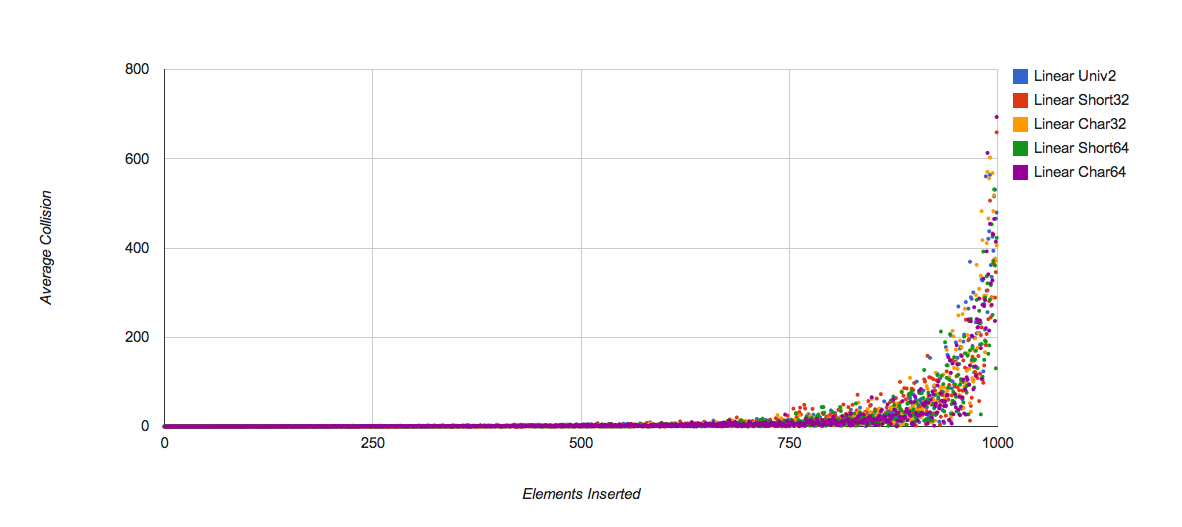
\includegraphics[width=\textwidth]{linear-collision.png}
                \caption{The average of number of collisions for different hash functions}
                \label{fig:linear-collision}
        \end{subfigure}
        

         \begin{subfigure}[b]{1\textwidth}
                \centering
                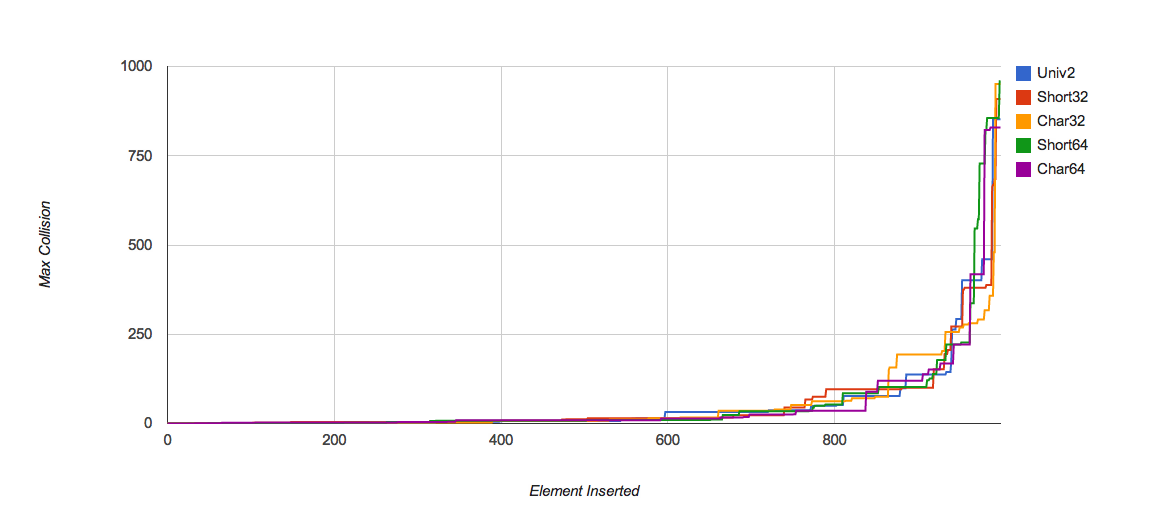
\includegraphics[width=\textwidth]{linear-max-query.png}
                \caption{The running maximum number of collisions for different hash functions}
                \label{fig:linear-max}
        \end{subfigure}
        \caption{Collision graphs for hash table with linear probing}\label{fig:linear}
\end{figure}


\subsubsection{Quadratic Probing}
Figure ~\ref{fig:quad} also shows that there is no significant 
between the different hash functions.


\begin{figure}
        \begin{subfigure}[b]{1\textwidth}
                \centering
                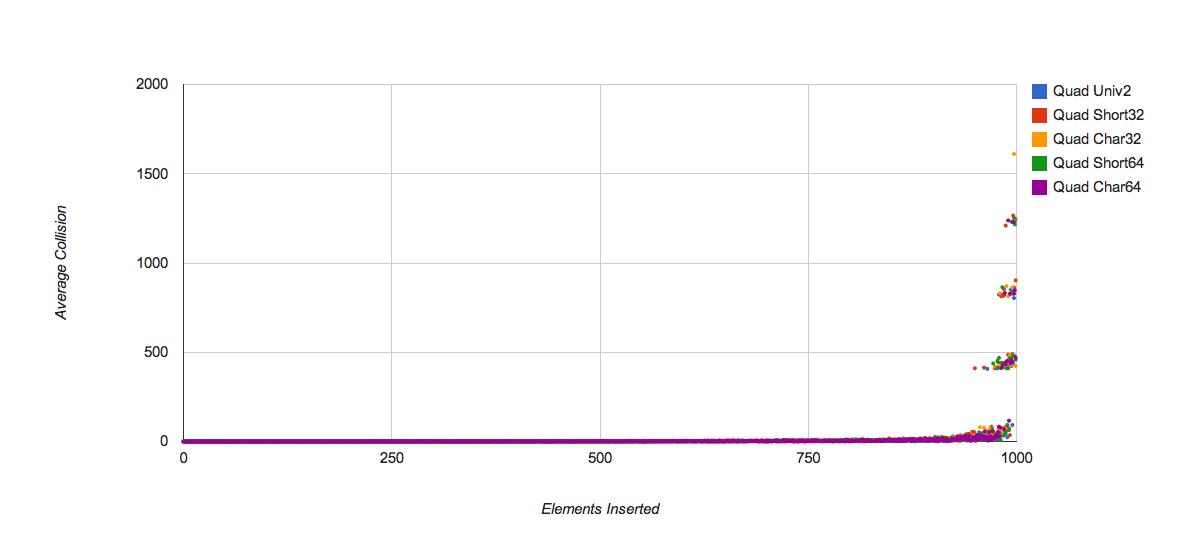
\includegraphics[width=\textwidth]{quad-collision.png}
                \caption{The average of number of collisions for different hash functions}
                \label{fig:quad-collision}
        \end{subfigure}       

         \begin{subfigure}[b]{1\textwidth}
                \centering
                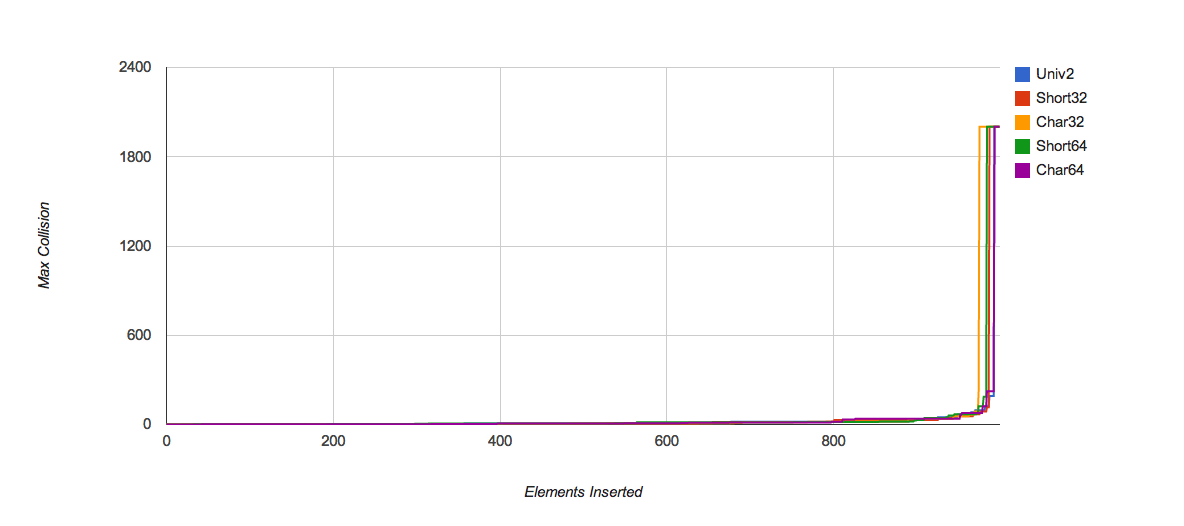
\includegraphics[width=\textwidth]{max-query-quad.png}
                \caption{The running maximum number of collisions for different hash functions}
                \label{fig:quad-max}
        \end{subfigure}
        \caption{Collision graphs for hash table with quadratic probing}\label{fig:quad}
\end{figure}


\subsubsection{Chaining}
While the number of collisions for the hash tables with chaining
is significantly lower, Figure~\ref{fig:chaining} shows a similar 
behavior between the different hash functions.


\begin{figure}
        \begin{subfigure}[b]{1\textwidth}
                \centering
                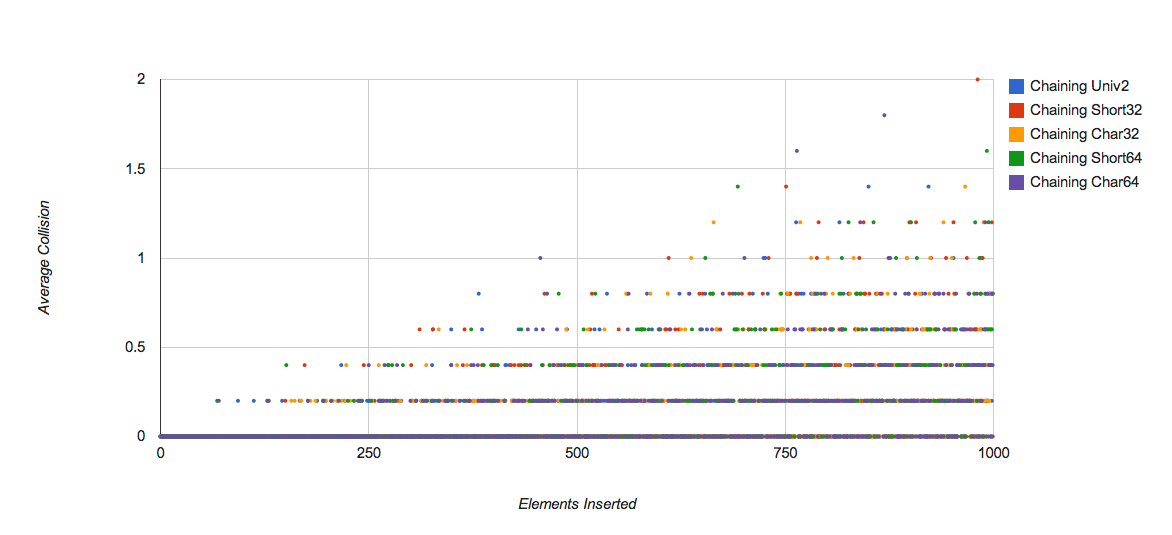
\includegraphics[width=\textwidth]{chaining-collision.png}
                \caption{The average of number of collisions for different hash functions}
                \label{fig:chaining-collision}
        \end{subfigure}

         \begin{subfigure}[b]{1\textwidth}
                \centering
                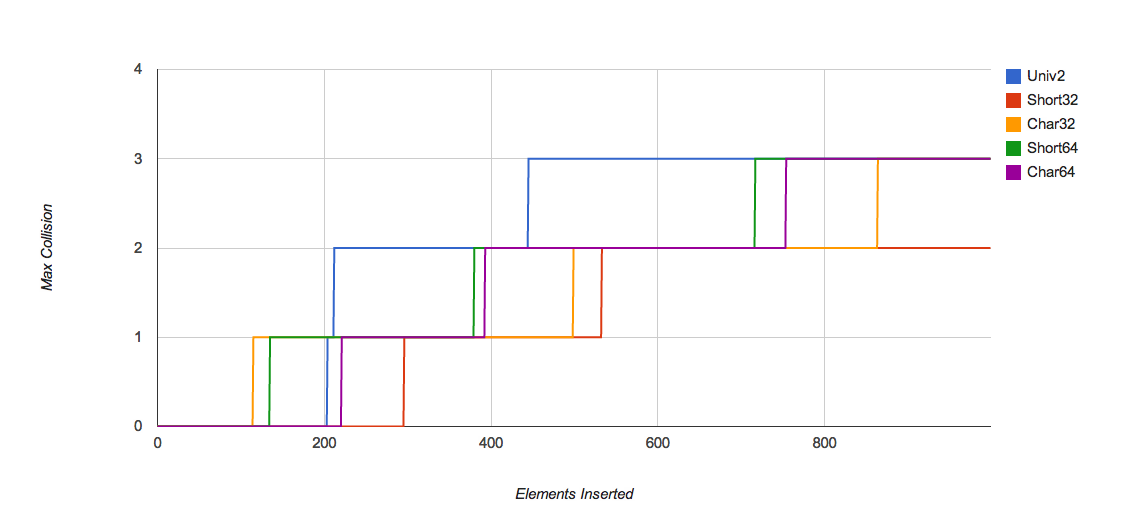
\includegraphics[width=\textwidth]{max-query-chaining.png}
                \caption{The running maximum number of collisions for different hash functions}
                \label{fig:chaining-max}
        \end{subfigure}
        \caption{Collision graphs for hash table with chaining}\label{fig:chaining}
\end{figure}


\subsubsection{Overall}
The comparison between the different collision resolution is much more interesting.
The results are shown in Figure~\ref{fig:collision}.
Throughout the benchmark test, chaining seems for perform much better than the other
two ways of collision resolution. It grows at much more linear rate. 
Aside from chaining, quadratic probing seems to be a little bit more 
efficient than linear problem. This is probably due to the fact that quadratic probing 
can be more resilient against clusters of occupied slots, by being able to jump over
the clusters more quickly. However, the average collision count spikes up to drastically
at a load factor of over 0.95. This is caused by the quadratic nature of the probing. Unlike linear
probing, quadratic probing can not guarantee to find an empty slot with number of probes
less than the table size. In order for the program to not stall, we had to cap the number of probes for quadratic probing to twice the size of the table.

\begin{figure}
        
                \centering
                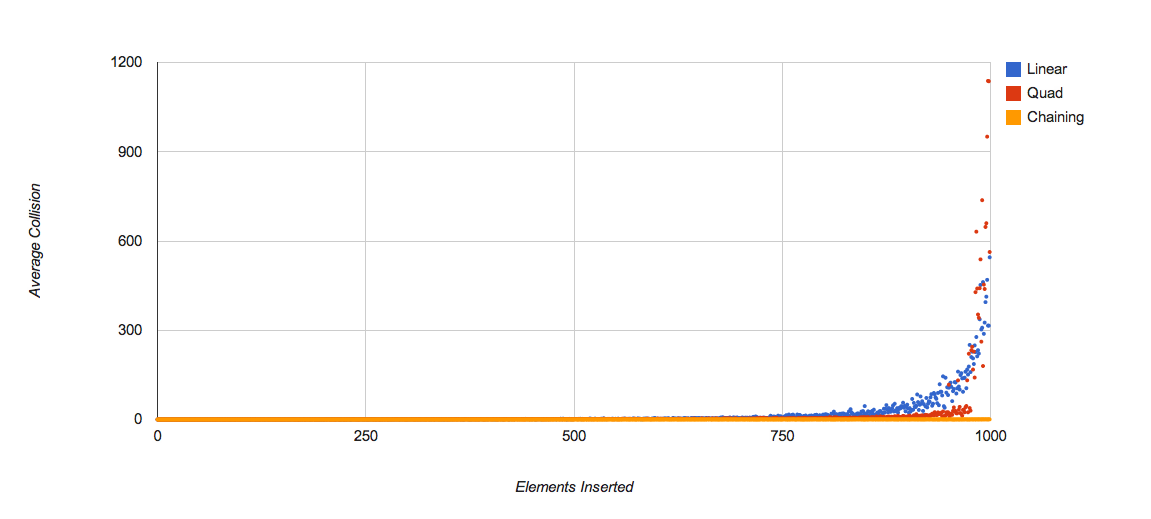
\includegraphics[width=\textwidth]{collision-all.png}
              \caption{The average number of collision with different collision resolution.}
              \label{fig:collision}
\end{figure}


\subsection{Time}

\subsubsection{Linear Probing}

\subsubsection{Quadratic Probing}

\subsubsection{Chaining}



Compare pure hashing vs tabulation hashing

compare linear probing

compare quadratic probing

compare chaining

compare between the three

some analysis on memory access  and mention pros ad cons of each


\section{Conclusion}
% Maksim
Thorup and Zhang analyzed in [1] how 5-independent Tabulation hashing's performance compared to the most basic Multiplication Based hashing method. In their paper they only used one type of collision resolution methods: linear probing. Following their results, we wanted to see how their results and claims project onto a larger set of experiments. We decided to compare the performance of Tabulation hashing described in their paper with the multiplication based hashing using 3 different collision resolution methods: linear probing, quadratic probing, and chaining. In the paper it is also mentioned that the same functions can be used to hash arrays of characters, or strings. We also decided to analyze how string hashing using 5-independent Tabulation hashing compares to hashing using multiplicative hashing. We implemented and ran a number of experiments to be able to compare all the methods. 





what we might do next
-maybe look at more specific timing data for when the table is really full
-also if we had time, we could have further optimized chaining by allocting many links in started 
instead of calling malloc 1000 times, which could be fairly slow.


\bibliographystyle{plain}
% Stuff will show up here if you use BibTeX
\begin{thebibliography}{77}

\bibitem{tz2010}
M. Thorup, Y. Zhang
\emph{Tabulation Based 5-Universal Hashing and Linear Probing},
2010

\bibitem{tz2004}
M. Thorup and Y. Zhang 
\emph{Tabulation Based 4-Universal Hashing with Applications to Second Moment Estimation},
Proc. 15th SODA:608-617 2004.
\bibitem{wc1981}
Mark N. Wegman and Larry Carter
\emph{New classes and applications of hash functions.},
Journal of Computer and System Sciences, 22(3):265 279, 1981. See also FOCS'79.
\end{thebibliography}

\bibliography{}

\end{document}

